\documentclass[a4paper,12pt]{report}
\usepackage[utf8x]{inputenc}
\usepackage[francais]{babel}
\usepackage[svgnames]{xcolor}
\usepackage{varioref}
\usepackage{textcomp}
\usepackage{graphicx}
\usepackage{tikz}
\usepackage{url}
\usepackage{ifthen}
\usepackage{xstring}
\usepackage{calc}
\usepackage{pgfopts}
\usepackage{titlesec}
\usepackage{listings}
\usepackage{hyperref}
\hypersetup{colorlinks=true, linkcolor=black}
\usepackage{color}

\lstset{ %
  language=C++,                     % the language of the code
  basicstyle=\footnotesize,       % the size of the fonts that are used for the code
  numbers=left,                   % where to put the line-numbers
  numberstyle=\tiny\color{gray},  % the style that is used for the line-numbers
  stepnumber=1,                   % the step between two line-numbers. If it's 1, each line
                                  % will be numbered
  numbersep=5pt,                  % how far the line-numbers are from the code
  backgroundcolor=\color{white},  % choose the background color. You must add \usepackage{color}
  showspaces=false,               % show spaces adding particular underscores
  showstringspaces=false,         % underline spaces within strings
  showtabs=false,                 % show tabs within strings adding particular underscores
  frame=single,                   % adds a frame around the code
  rulecolor=\color{black},        % if not set, the frame-color may be changed on line-breaks within not-black text (e.g. commens (green here))
  tabsize=2,                      % sets default tabsize to 2 spaces
  captionpos=b,                   % sets the caption-position to bottom
  breaklines=true,                % sets automatic line breaking
  breakatwhitespace=false,        % sets if automatic breaks should only happen at whitespace
  title=\lstname,                 % show the filename of files included with \lstinputlisting;
                                  % also try caption instead of title
  keywordstyle=\color{blue},      % keyword style
  commentstyle=\color{magenta},   % comment style
  stringstyle=\color{red},      % string literal style
  escapeinside={\%*}{*)},         % if you want to add a comment within your code
  morekeywords={*,...}            % if you want to add more keywords to the set
} 

\bibliographystyle{plain}
\frenchbsetup{StandardLists=true}

%%%%%%%%%%%%%%%%%%%%%%%%%%%%%%%%%%%%%%% PDF INFO 
%%%%%%%%%%%%%%%%%%%%%%%%%%%%%%%%%%%%%%%%%%%%%%%%
\hypersetup{
	pdfauthor   = {Rémy François, Damien Druel, Erwan Douaille et Yoan Miranda},
	pdftitle    = {Rapport de Projet Scientifique},
	pdfsubject  = {Kinect interraction},
	pdfkeywords = {Rémy François Damien Druel Kinect Erwan Douaille Yoan Miranda Lille},
	pdfcreator  = {PDFLaTeX},
	pdfproducer = {PDFLaTeX}
}
%%%%%%%%%%%%%%%%%%%%%%%%%%%%%%%%%%%%%%%%%%%%%%%%

\author{Rémy François, Damien Druel, Erwan Douaille et Yoan Miranda}
\title{}
\titleformat{\chapter}[hang]{\bf\huge}{\thechapter}{2pc}{}


\begin{document}

\makeatletter
\begin{titlepage}
\centering
\vspace{-10em}
{\LARGE \textbf{\textsc{Rapport de Projet RVI}}}\\
\vspace{3em}

\includegraphics[scale=0.6]{image/thalassa.png}\\
\vspace{3em}
{\LARGE \textsc{Projet Thalassa: simulation de plongée sous-marine}}\\

\vspace{8em}
Par\\
\vspace{1em}
{\LARGE \@author}\\

\vspace{2em}



\begin{tikzpicture}[remember picture,overlay]

\node [below left,xshift=-1cm, yshift=4cm] at (current page.south east){
\includegraphics[scale=0.6]{image/ustl1.png}};

\end{tikzpicture}
\end{titlepage}
\makeatother

\sloppy
\thispagestyle{empty}
\chapter*{Remerciements}

Je tiens à remercier l’ensemble des membres de l'équipe MINT/PIRVI pour m’avoir accueillis dans la bonne humeur et pour avoir partagé avec moi leurs savoirs.

J’aimerais tout particulièrement remercier Samuel Degrande et Laurent Grisoni pour m’avoir apporté les conseils et connaissances, qui m’ont aidé tout au long de ce stage.

Je remercie finalement, l’ensemble des enseignants du Master informa
tique, pour m’avoir apporté les compétences nécessaires pour accomplir ce stage.
\newpage

\thispagestyle{empty}
\chapter*{Résumé}

TODO ?

\thispagestyle{empty}

\tableofcontents
\thispagestyle{empty}
\newpage
\setcounter{page}{1} 

%%%%%%%%%%%%%%%%%%%%%%%%%%%%%%%%%%%%%%% contenu futur
\chapter{Introduction}

Avec la montée en puissance de calcul des processeurs graphiques (GPU) le monde de l'imagerie a ces vingts dernières années énormément évolué. L'une de ces évolutions est l'apparition d'écran large. Les écrans larges d'il y a dix ans, qui représentent des écrans 21"\cite{Czerwinski:2006:LDR:1125451.1125471}, sont aujourd'hui très courants dans le milieu des ordinateurs de bureau et sont souvent utilisés en multi-monitoring. Notre définition d'écrans larges correspond à des murs, soit des écrans par exemple de quatre mètres de large pour deux mètres de haut. Alors que Czerwinsky et al.\cite{czerwinski2003toward} démontrent que les écrans d'une vingtaine de pouces apportent un gain de confort, de performance et de précision dans l'utilisation des ordinateurs, on remarque que pour des écrans larges faisant la taille d'un mur ce constat n'est plus valable. Comme visible dans de nombreuses études \cite{Schmidt:2013:SEP:2470654.2466227, Vogel:2004:IPA:1029632.1029656, jakobsen2013information} les écrans larges apportent de nouvelles questions comme, comment interagir avec des grands écrans, comment afficher une image pour différents points de vue, ou encore comment apporter un confort visuel aux personnes ayant des troubles visuels tout en utilisant de grands écrans. L'interaction et l'appréhension de l'image sur écran géant sont différentes de ce que l'on rencontre sur des écrans classiques d'une vingtaine de pouces.

\section{Problématique} 

Deux problèmes en particulier apparaissent lors de l'utilisation d'écrans géants. L'un étant que lorsque l'utilisateur est proche de l'écran un effet de perspective apparaît ce qui pose problème pour interagir avec ce qui est situé aux bords de l'écran. Le second problème est lors d'une interaction distante, à cause de la grande densité de pixel que l'écran fournit, il est difficile de voir tout les détails de l'écran ce qui apporte une difficulté et une imprécision dans l'interaction.

Pour répondre à ces deux problèmes, deux solutions sont envisageables. La première est de travailler sur la partie interaction pour permettre d'aider l'utilisateur à mieux interagir avec ces grands écrans. La seconde solution est de déformer l'image pour obtenir une taille d'affichage cohérente avec les capacités d'interaction. Dans cette étude nous travaillerons sur la seconde solution qui est la déformation d'image.

Nous verrons donc comment correctement déformer l'image en tenant compte de la position de l'utilisateur face à l'écran pour lui fournir la meilleure interaction possible.


%
%\chapter{Introduction}
%
%Une anamorphose est une déformation réversible d'une image à l'aide d'un système optique, tel un miroir courbe, ou un procédé mathématique. Le but de ce projet est d'étudier l’anamorphose dite dynamique qui fut introduite pour la première fois en 2007 par Solina, F. et Batagelj, B \cite{dynamicAnamorphosis}. L’aspect dynamique de l’anamorphose consiste à ne pas appliquer une déformation statique de l’image, mais à déformer l’image en temps réel en tenant compte de paramètres tels que la position de l’utilisateur face à l’image. 
%
%\section{Contexte}
%
%Ce projet, se basant sur l’anamorphose dynamique de Solina, F. et Batagelj, B \cite{solina2007dynamic}, consiste à appliquer l'anamorphose à un système d'exploitation autrement dit, à un ordinateur avec lequel l’utilisateur peut interagir. Dans notre cas, l'ordinateur utilise un écran géant de 2 mètres de haut sur 4 mètres de largeur. Face à un tel écran l'utilisateur voit apparaître un effet de perspective lorsque celui-ci est très proche de l’écran et qu’il souhaite regarder les éléments qui sont présents au bord de l’écran.
%
%\section{Problématique} 
%
%L'objectif principal de ce projet est de pouvoir apporter un confort visuel à l'utilisateur. Cet objectif vise à corriger l'effet de perspective qui pourrait apparaître sur des écrans géants ou encore apporter une facilité visuelle d'interaction avec ce type d'écran qui possède une densité de pixel par pouce élevé et pour lesquels les systèmes d'exploitation moderne ne sont aujourd'hui pas adaptés. 

\section{Plan du projet}

Dans un premier temps, un état de l'art présente ce qui a déjà été réalisé autour de la déformation d'image ainsi que des techniques pour apporter du confort visuel. Une seconde partie concerne les contributions apportées par cette étude: proposition d'un cadre logiciel permettant la déformation totale ou partielle de l'image tout en conservant les propriétés d'interaction,  et la mise en œuvre sur deux cas d'usage. Ce rapport se finit par une conclusion et des perspectives sur la suite de ce travail sont proposées.
\chapter{Présentation de l’application et de ses fonctionnalités}

L’application que nous devons enrichir á été développé par Hanaë Rateau dans le cadre de son doctorat au sein de l’équipe MINT. Cette application consiste à traquer, via la Kinect, un ou plusieurs utilisateurs et leurs permettre de créer des espaces d’interactions pour pouvoir contrôler à distance la souris de l’ordinateur sur plusieurs écrans.

\section{Espace d’interaction virtuel}

L’espace d’interaction virtuel, comme décrit dans l'article de \textit{Rateau et al.} \cite{rateau:hal-00851935},  est une notion qui consiste à réserver une partie de l’espace de l’utilisateur pour interagir. Cet espace d’interaction peut être de différentes dimensions comme une courbe, une surface plane ou un volume.  Dans l’application, cet espace virtuel est utilisé pour contrôler le curseur de la souris sur plusieurs écrans (en mode bureau étendu). L’utilisateur peut changer d’écran en faisant un geste partant de l’espace vers l’écran concerné. Pour l’instant, il n’est possible de travailler que sur 2 écrans positionnés à des endroits fixes. Pour créer un espace d’interaction virtuel, l’utilisateur doit dessiner un carré dans l’espace. 
	 
\begin{figure}[!ht]
	\center	
	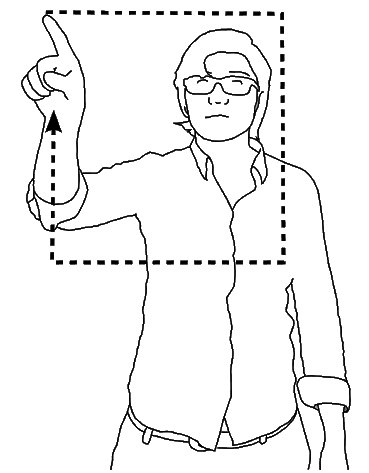
\includegraphics[scale=0.2]{image/create.png}
	\caption{Création de l'espace d'interaction virtuel}
\end{figure}

Cet espace virtuel ne peut pas être déplacé par les utilisateurs mais peut être supprimé par un mouvement rapide ayant pour représentation de pousser l’espace virtuel.

\begin{figure}[!ht]
	\center	
	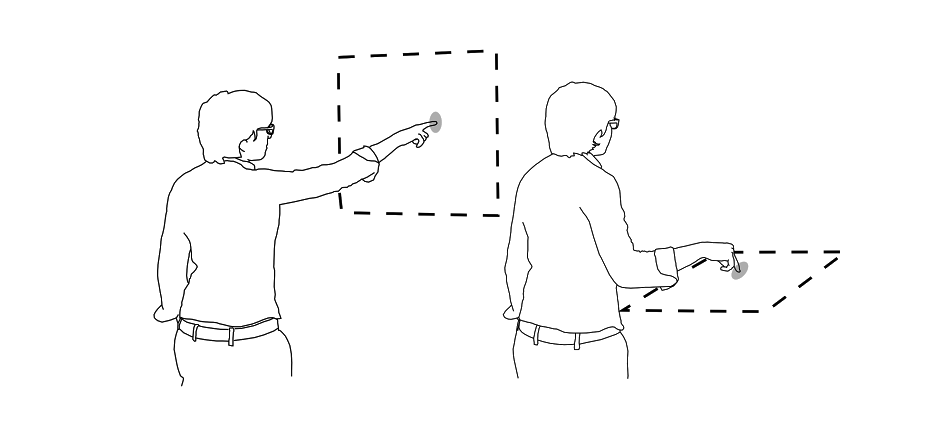
\includegraphics[scale=0.3]{image/touch.png}
	\caption{Représentation de l'espace d'interaction virtuel}
\end{figure}

Dans cet espace, il faut traquer la position de la main de l’utilisateur pour pouvoir mettre à jour la position de la souris et permettre la reconnaissance de gestes afin de savoir quand supprimer l’espace d’interaction virtuel concerné.

\begin{figure}[!ht]
	\center	
	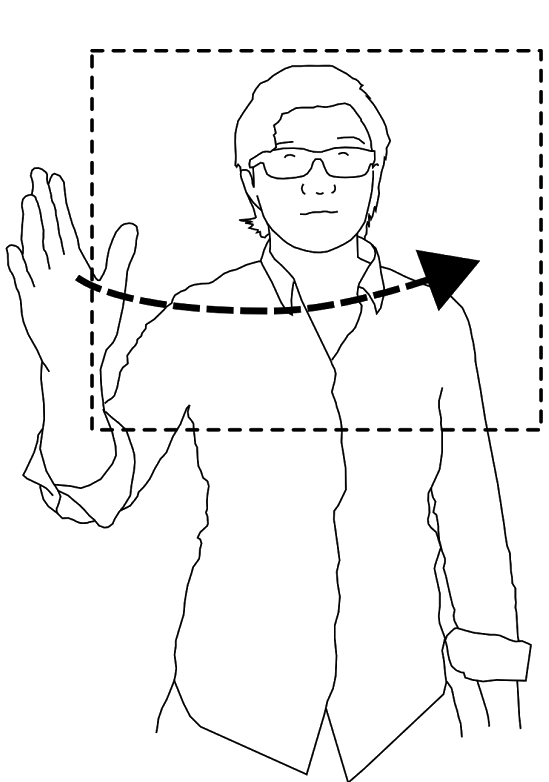
\includegraphics[scale=0.2]{image/remove.png}
	\caption{Suppression de l'espace d'interaction virtuel}
\end{figure}
	
\newpage

\section{Kinect}

La Kinect est un outil développé par l'entreprise PrimeSense et popularisé par Microsoft avec la Xbox 360, qui l’utilise comme un periphérique de jeu permettant de jouer sans manette. Ce dispositif possède une caméra couleur ainsi qu’une caméra et un émetteur infrarouge. L’émetteur envoie des rayons infrarouges structurés ce qui permet, à l’aide de la caméra infrarouge, d’obtenir des informations sur la profondeur de l’image acquise en analysant la projection des points. 

\begin{figure}[!ht]
	\center	
	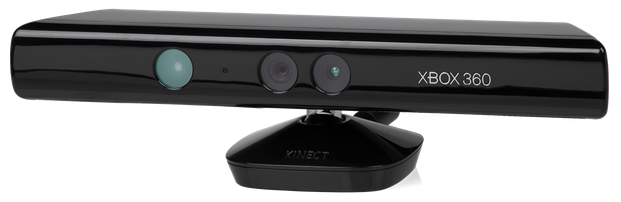
\includegraphics[scale=0.5]{image/kinect.png}
	\caption{La Kinect}
\end{figure}

Grâce à ces images, nous pouvons obtenir des données sur la position dans un environnement en 3D des différents membres des utilisateurs et donc de reconnaitre les mouvements effectués par l’utilisateur. 

La caméra Kinect possède un taux d'acquisition de 30 images par seconde avec une résolution de 640x480 pixels. Le capteur capte avec une portée minimale de 0.5 mètre et peut acquérir des objets situés jusqu’à 3.5 mètres dans un champ de vision horizontal de 57° et de 43° en vertical.

L'ajout du contrôle via Kinect est pertinent puisqu'il s'agit d'un outil grand public et à faible coût, contrairement a des solutions plus performantes, comme les ARTrack, qui ont un coût élevés et qui demande une calibration ainsi qu’un équipement des utilisateurs avec les dispositifs nécessaires.

Dans le cas de notre projet, la Kinect est utilisée pour tracker les personnes et plus particulièrement la position et l’orientation de leurs mains. Ces données sont envoyées via un serveur TUIO modifié. Pour que la Kinect soit plus performante le 1€ filter \cite{oneeuro} est utilisé pour supprimer le bruit et d’obtenir un pointeur virtuel plus stable. 



\section{Problématiques}

\subsection{Visualisation de l’espace virtuel}

Le problème qui se pose avec l’utilisation de l’espace virtuel est l’absence de retour visuel pour l’utilisateur ainsi que le manque de retour physique indiquant une action effectué. Dans notre cas nous avons un retour visuel car nous travaillons sur un prototype. Cependant, dans le cadre d’une utilisation grand public, l’utilisateur n’aura plus ce retour visuel. Il ne pourra pas avoir d’information sur l’emplacement de l’espace virtuel ni de la position de sa main par rapport à celui-ci.

\begin{figure}[!ht]
	\center	
	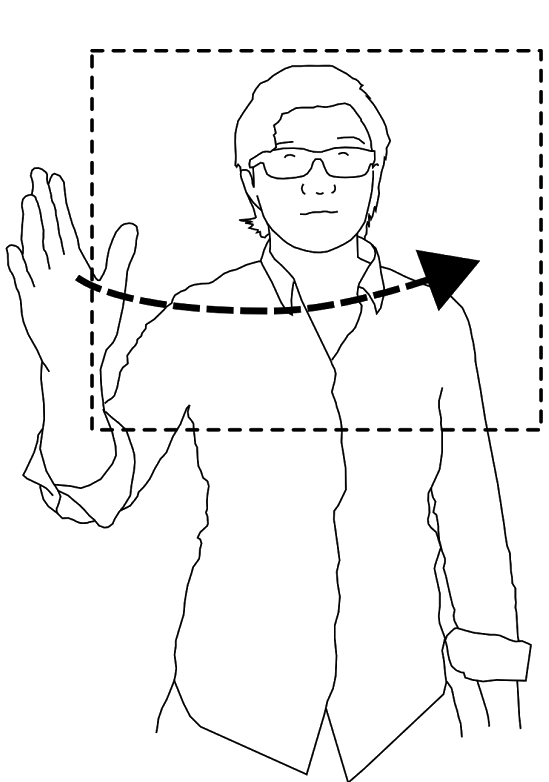
\includegraphics[scale=0.2]{image/remove.png}
	\caption{Visualisation de l'espace d'interaction virtuel}
\end{figure}

Ce manque d’information est troublant à l’utilisation. De plus lors d’une utilisation en multi-utilisateur, l’action de transmettre l’espace virtuel ou simplement de le localiser est complexe voir impossible. (citer article) La possibilité de pouvoir attacher un espace à un objet physique permettrait de résoudre ce problème de visualisation.


\subsection{Occlusion de la main par le support physique}

Dans le cas ou on utiliserait un support physique, plusieurs questions se posent sur l’occlusion. 
Le support peut dans certaines orientations empêcher le tracking de la main de l’utilisateur. Pour pallier à ce problème il faut, soit demander à l’utilisateur de tenir le support à plat face à la kinect, ce qui n’est pas confortable, ou placer plusieurs Kinect.
L’ajout de Kinects, ou de webcams supplémentaires peut nous permettre de visualiser la scène sous plusieurs angles et donc de suivre la main même quand celle-ci n’est pas visible par la Kinect principale.  

\subsection{Partage de l’objet virtuel}

Comme cité précédemment, le dernier problème est la difficulté pour partager l’objet virtuel. En effet, l’utilisateur courant doit sortir de l’espace virtuel puis le deuxième utilisateur doit rentrer dans cet espace pour effectuer le partage ce qui suppose que le deuxième utilisateur arrive à situer parfaitement l’espace virtuel dans le monde réel. Avec un support physique, il suffirait de partager le support pour partager l’espace virtuel par la même occasion.  

\chapter{État de l’art}

\section{Introduction}

Comme cité précédemment, les écrans géants sont une technologie qui tend à se répandre et à être de plus en plus présent dans notre environnement. Cependant l'utilisation et l'appréhension de cet outil est différent de ce que l'on peut rencontrer actuellement sur des écrans dits classiques. Notre étude des écrans géants se porte sur l'amélioration du confort visuel pour un utilisateur en fonction de sa distance avec l'écran. En effet, en fonction de la distance qui sépare l'utilisateur de l'écran, l'interaction et le ressenti visuel sont différents. Sur une interaction dite proche un effet de perspective apparaît et devient gênant pour interagir avec les widgets visibles sur l'écran. Sur une interaction éloignée la densité d'information visuelle est un inconvénient pour une interaction précise.

\section{Interaction proche sur grand écran}

\subsection{Effet de perspective}

La perspective est l'un des indices visuels qui nous permet de représenter le monde qui nous entoure. La perspective est un ensemble de règles énoncées par \textit{Filippo Brunelleschi} qui permet de représenter une image sur une surface plane tout en ayant l'impression de réalité grâce à des lignes de fuite. Les lignes sont des ensembles de points qui représentent la direction du plan visualisé. Celles-ci sont présentes lorsque l'on regarde un écran géant de près et donne un rendu étiré de l'image qui est affichée dans notre cas, sur l'écran géant. Voici un aperçu de ce qu'est l'effet de perspective rencontré face à une surface plane, voire figure \ref{fig:perspectiveScreen}, ce qui est également ce qu'on obtient face aux écrans géants.

\begin{figure}[!ht]
	\center	
	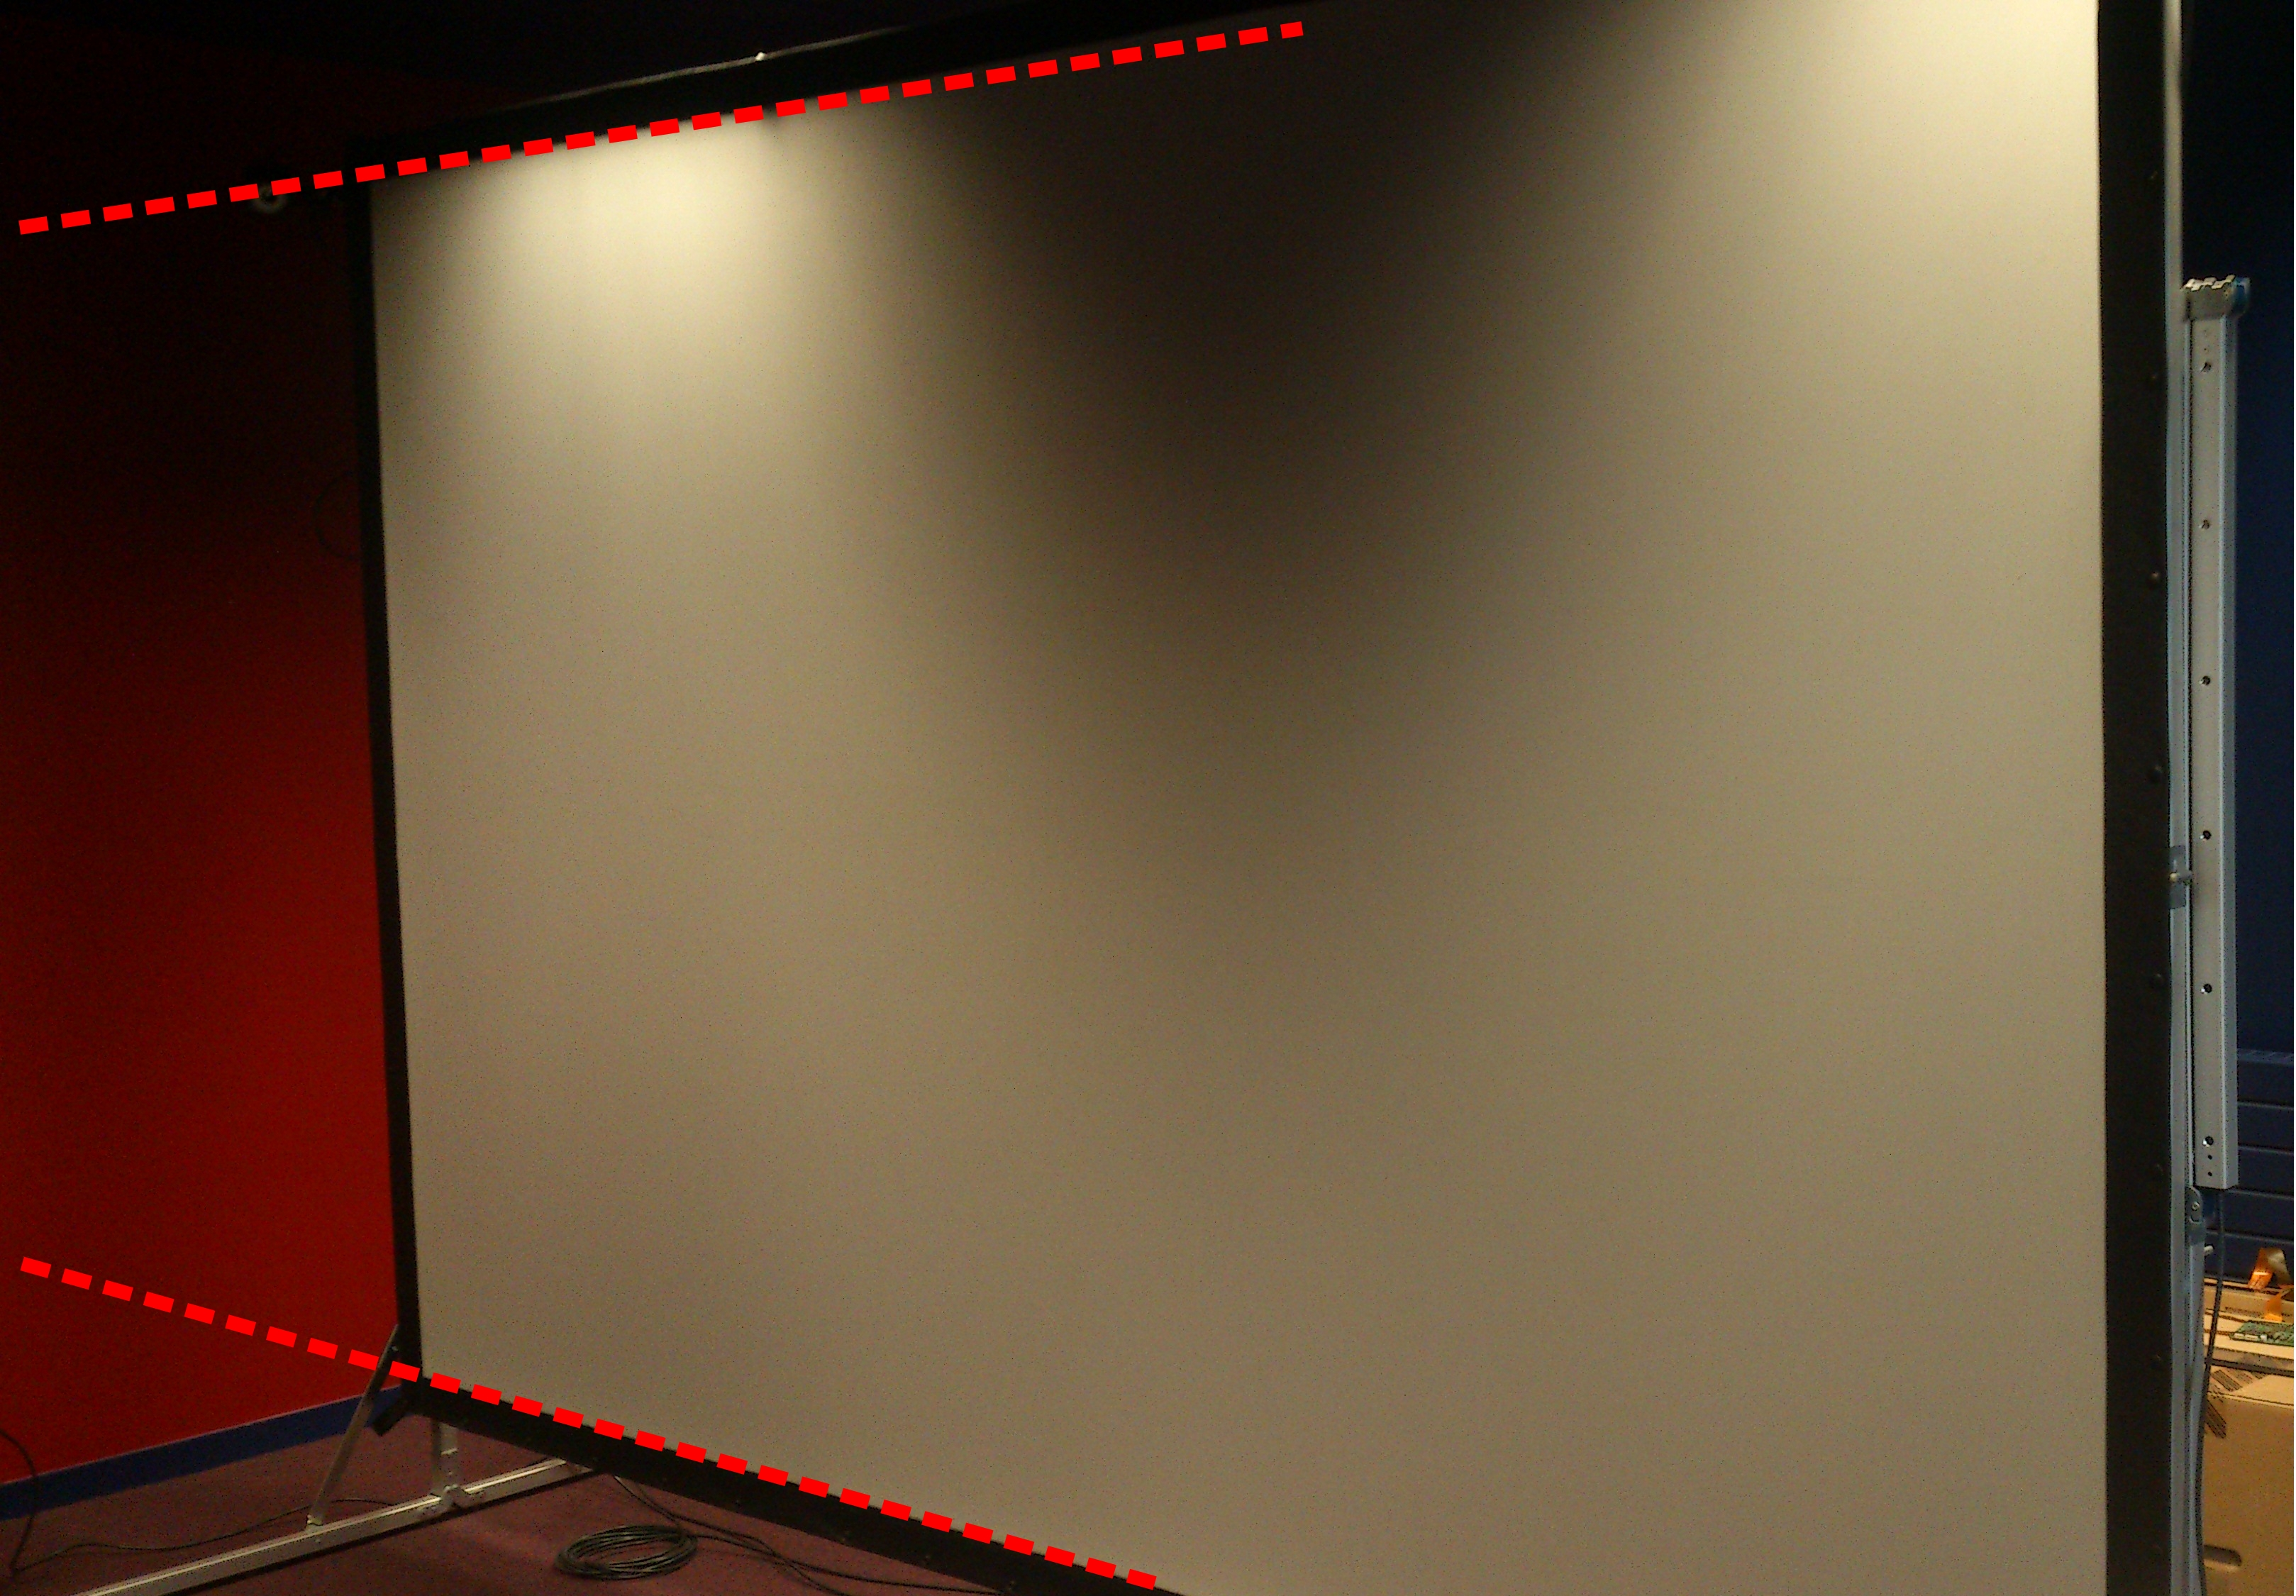
\includegraphics[scale=0.1]{image/perspectiveScreen.jpg}
	\caption{Effet de perspective visible face à un écran géant}
	\label{fig:perspectiveScreen}
\end{figure}

L'effet de perspective est un sujet qui a été traité dans de nombreux cas comme par exemple avec Econics \cite{Nacenta:2007:EPI:1294211.1294260} qui traitait le problème de l'effet de perspective par une déformation statique des fenêtres de l'environnement. 

\subsection{Correction de la perspective}


Econics voire figure \ref{fig:econics}, est un prototype permettant de définir plusieurs écrans situé a des emplacements et orientation aléatoire tout en proposant pour l'utilisateur un retour visuel de son application orthogonal par rapport à son point de vue et non par rapport à l'écran.

\begin{figure}[!ht]
	\center	
	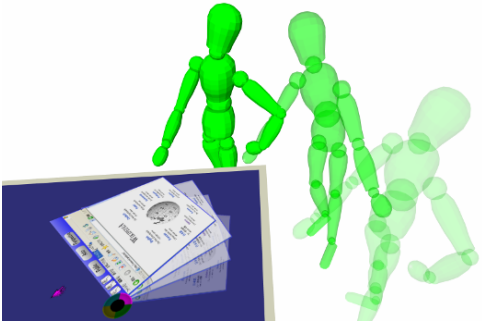
\includegraphics[scale=0.5]{image/econics.png}
	\caption{Aperçu de la correction de perspective d'Econics}
	\label{fig:econics}
\end{figure}

Comme Econics l'a fait pour corriger l'effet de perspective, il est possible de modifier la géométrie des fenêtres affichées de façon indépendante les unes des autres. Econis fait une déformation dynamique des fenêtres en fonction du point de vue utilisateur. La déformation de la fenêtre sur fait autour d'un point d'ancrage 3D que l'utilisateur définit. Econics introduit donc une base à la correction de la perspective cependant il a été conçu pour répondre à la problématique de la correction de perspective sur plusieurs écrans de taille normale dispersés dans une pièce et non un unique écran géant. 
%% il y a une déformation dynamique fonction du pt de vue utilisateur indé pour chaque fenetre. Chaque fenetre tourne autour d'un point d'acnreage 3D définit pour l'utilisateur OK

La correction de perspective a également été mise en place pour le prototype Screenfinity \cite{Schmidt:2013:SEP:2470654.2466227} réalisé par Schmidt et al. . L'objectif de Screenfinity est d'afficher du texte déformé sur un écran géant pour que les passants puissent lire le texte tout en marchant et sans l'effet de perspective, voire figure \ref{fig:screenfinity}. Screenfinity utilise donc la déformation dynamique d'image en tenant compte de la position des passants et de leurs orientation de tête. Pour calculer la déformation à appliquer, la position et l'orientation des passant sont pris en compte. Cette déformation de l'image prend en considération les caractéristiques de la vision humaine.
%% Cette déformation prend en compte les caractéristiques de la vision humaine
%Pour calculer la déformation à appliquer en fonction de la position et l'orientation des passant, il faut tenir compte de l'acuité visuelle. OK

\begin{figure}[!ht]
	\center	
	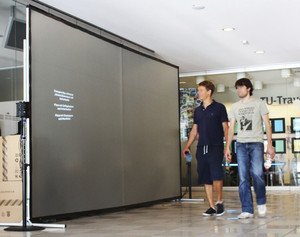
\includegraphics[scale=1]{image/screenfinity.jpg}
	\caption{Aperçu de Screenfinity et de sa correction de perspective en fonction du regard des passants}
	\label{fig:screenfinity}
\end{figure}


\subsection{Méthode de déformation d'affichage}

L'une des méthode générique de déformation d'image est l'anamorphose découverte fin du quinzième siècle dans le milieu de l'art tant pour ajouter du challenge aux artistes que pour confirmer leurs maîtrises de la perspective qui fût découverte en même temps.
Une anamorphose est une déformation réversible d'une image à l'aide d'un système optique, tel un miroir courbe, ou un procédé mathématique.

L'une des plus célèbres anamorphoses est celle réalisée par Hans Holbein sur la toile \textit{Les ambassadeurs}, voir \ref{fig:ambassador}.

\begin{figure}[!ht]
    \centering
    \subfigure[]{\label{sub1} 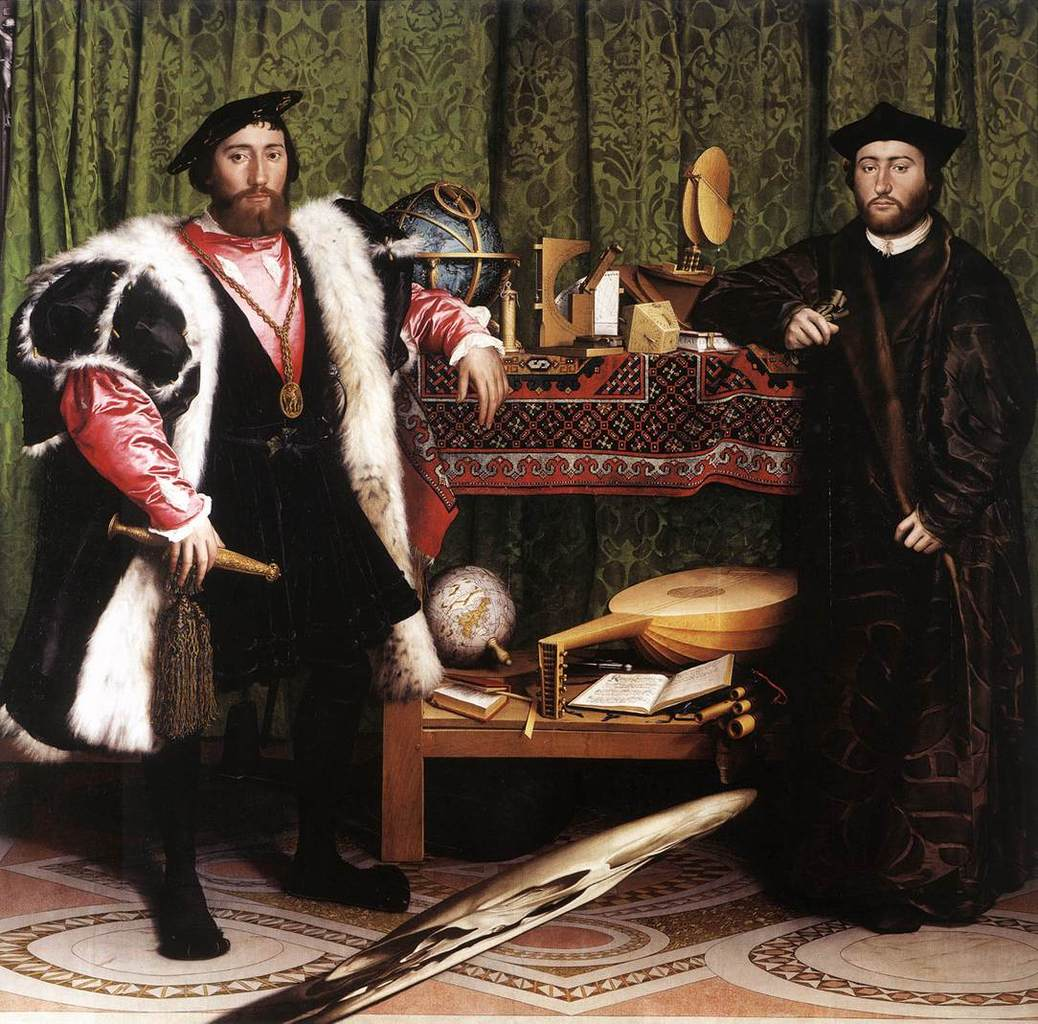
\includegraphics[scale=0.7]{image/ambassador.jpg}}
    \subfigure[]{\label{sub2} 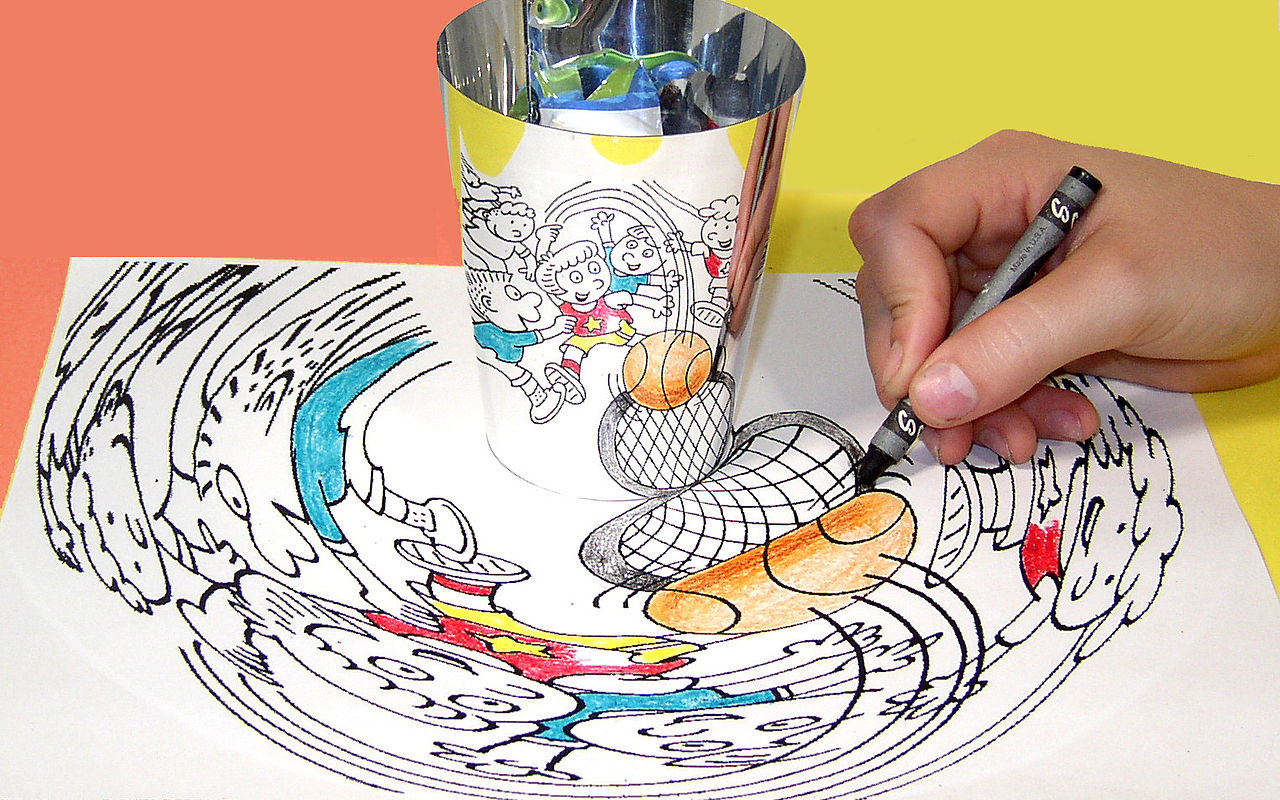
\includegraphics[scale=0.2]{image/anamorphose}}
    \caption{Les ambassadeurs de Hans Holbein le Jeune, 1533 \subref{sub1},  anamorphose avec miroir cylindrique \subref{sub2}.}
	\label{fig:ambassador}
\end{figure}

Sur cette toile, on peut voir apparaître une forme étrange sur le bas de ce tableau, il s'agit d'une anamorphose d'un crâne humain. Si on regarde le tableau depuis le côté inférieur gauche du tableau, le crane est visible correctement. L'anamorphose est présente sur plusieurs supports, comme par exemple dessiné par des artistes dans certaines rues \cite{pavementArt}.

%% enlever premiere et derniere OK
L’aspect dynamique de l’anamorphose consiste à ne pas appliquer une déformation statique de l’image, pour laquelle il faut se placer à un point de vue particulier pour obtenir visuellement l'image non déformée, mais déformer l’image en temps réel en tenant compte de paramètres, tels que la position de l’utilisateur face a l’image, pour que celle-ci soit déformée mais parfaitement visible pour l'utilisateur. 

L'anamorphose dynamique introduite par Solina et al. est de la distorsion d'image pour afficher des visages tout en ayant l'impression que le regard des portraits est dirigé vers l'utilisateur. Nous reprendrons donc l'idée de la déformation dynamique sans conserver l'objectif de Solina et al. qui était de garder la direction du regard du portrait vers l'utilisateur.










\section{Interaction distante sur grand écran}
%%changer le titre pour perception humaine OK
\subsection{Perception humaine}

L'acuité visuelle est la mesure de la résolution spatiale du processus visuel, autrement dit de l'œil humain. La vision binoculaire est un mode de vision dans lequel les deux yeux sont utilisés simultanément \ref{fig:acuite}. 

\begin{figure}[!ht]
	\center	
	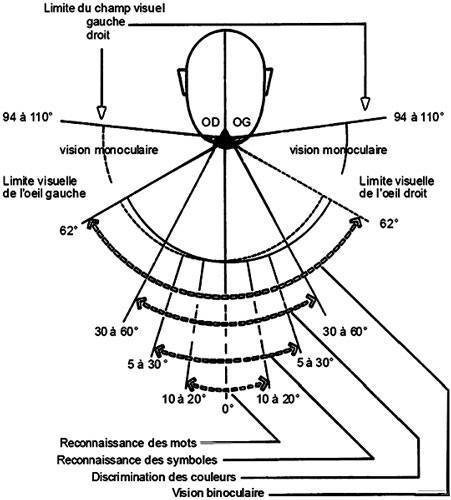
\includegraphics[scale=0.4]{image/acuite.jpg}
	\caption{Représentation des différents champs de vision de l'être humain.}
	\label{fig:acuite}
\end{figure}
%% elevé du détail sur chaque oeil, juste préciser le 120 binoculaire + capacité vison de détail OK
Les humains ont un champ de vision horizontal maximal de $\simeq$120\degres  environ avec les deux yeux. La vision humaine est également limité en terme de perception des détails. En moyenne un œil humain n'arrive pas à percevoir une différence au delà de 76 dpi à une distance de un mètre, et au delà de 38 dpi pour une distance de deux mètres. Il faut donc tenir compte de la vision humaine lorsque l'on fait de l'affichage.

%% changer : la vision humaine doit être prise en compte lorsque l'on fait de l'affichage. OK
%L'acuité visuelle est également importante dans le cas ou la densité d'affichage est élevé et que l'on souhaite lire à distance des informations. 


Comme dit précédemment les écrans sont de plus en plus grands et leurs résolutions sont également de plus en plus élevées. Trois problèmes liés à l'augmentation du nombre de pixel présent par unité d'espace, autrement appelé pixel per inch (ppi) sont présentés selon Agarwal et al. \cite{Agarwal:2013:WSA:2578048.2578052}. Sur les trois problèmes identifiés deux nous concernent directement pour l'utilisation distante des grands écrans.

Le premier problème étant que la plupart des applications, les systèmes d'exploitation et plus généralement les interfaces graphiques ne sont pas adaptés pour des résolutions élevées. Ce fut le cas des écrans "Retina" (220 ppi) d'Apple qui ont dû forcer certaines applications à se mettre à jour car inadapté pour une telle résolution, habituellement comprise entre 72 et 110 dpi. Ensuite vient le problème lié à la vision des utilisateurs. En effet les utilisateurs ayant des troubles de la vision, tels que les daltoniens ou encore les personnes âgées, souffrent des mêmes problèmes face à des écrans avec de grandes résolutions d'affichages. Ces problèmes sont des incapacités à lire correctement du texte, une imprécision sur l'ensemble des images affichées à l'écran, ou encore une incapacité à interagir avec des widgets trop petits.

En effet, comme expliqué dans cet article \cite{Nancel:2013:HPL:2470654.2470773} qui traite d'une technique d'interaction pour grands écrans, lorsqu'il y a interaction directe avec l'écran la zone sous le doigt correspond a une douzaine de pixel. On imagine bien que le problème du pointage à distance qui en plus d'être imprécis, apporte encore plus de difficultés pour interagir avec une zone comportant énormément de pixels.
          
\subsection{Zoom global}


Pour palier à ces problèmes d'affichage trop petit une solution fut d'utiliser les loupes \cite{Kline:1995:IGA:223904.223919}, autrement appelées magnifying glass.

\begin{figure}
    \centering
    \subfigure[]{\label{sub1} 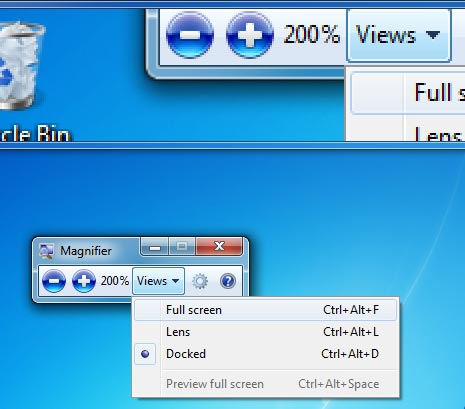
\includegraphics[scale=0.4]{image/loupeWindows.jpg}}
    \subfigure[]{\label{sub2} 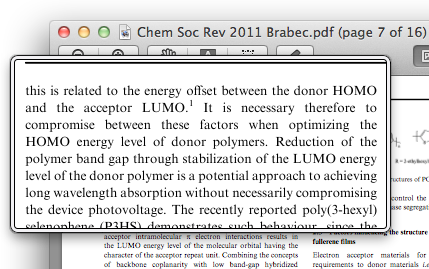
\includegraphics[scale=0.4]{image/loupeMac.png}}
    \caption{Aperçu des loupes implémentés dans \subref{sub1}Windows et \subref{sub2}Mac OS X.}
	\label{fig:loupeDemo}
\end{figure}

Parmi les loupes existantes et implémentées dans les systèmes d'exploitation modernes, la plupart occupent l'ensemble de l'écran ou cachent certaines parties autour de la loupe, voir figure \ref{fig:loupeDemo}. Cela à pour effet de perdre une partie des informations se trouvant sous les bords de la loupe. Pour les loupes qui occupent une plus grande partie de l'écran, cela a pour effet de perdre encore plus d'informations car si l'utilisateur n'a pas connaissance de son environnement graphique, il doit parcourir l'ensemble de l'écran pour pouvoir s'y repérer et interagir. 


\subsection{Zoom local}

Pour garder une vue globale de l'environnement graphique de nombreuses loupes ont étés expérimentés \cite{Carpendale:2004:AHM:1029632.1029645}, voire un aperçu des loupes figure \ref{fig:loupeMultiple}. Ces loupes permettent de faire un zoom sur l'image sans cacher l'information autour ou en dessous du zoom. Ce sont des zooms de type local.


\begin{figure}[!ht]
	\center	
	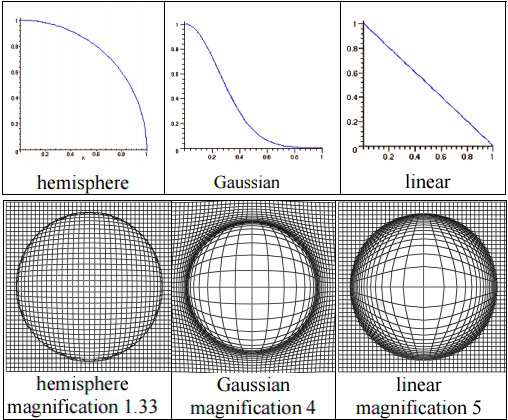
\includegraphics[scale=0.7]{image/LoupeMultiple.png}
	\caption{Aperçu de différents types de loupe}
	\label{fig:loupeMultiple}
\end{figure}

% demo fisheye
L'une des loupes qui ré-apparaît souvent dans la littérature est la loupe fisheye, voire figure \ref{fig:fisheyeMap}

\begin{figure}[!ht]
	\center	
	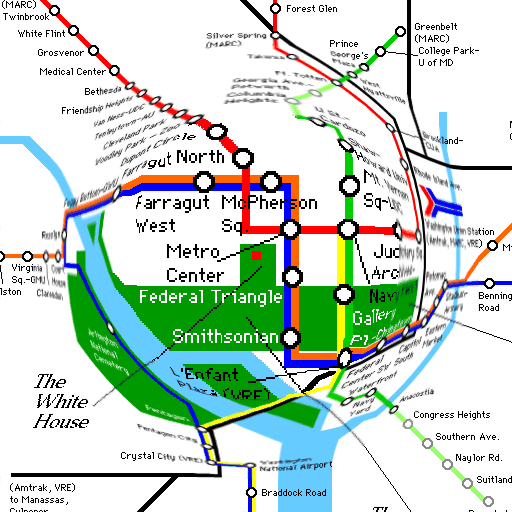
\includegraphics[scale=0.4]{image/fisheyeMap.png}
	\caption{Carte avec rendu fisheye}
	\label{fig:fisheyeMap}
\end{figure}

Dans le domaine de l'interaction homme machine la question du zoom fisheye a souvent été étudié \cite{Shneiderman:1986:DUI:6682, Ware:1995:DIM:223355.223749, Cockburn:2009:ROZ:1456650.1456652} et mis en avant pour montrer l'avantage de cette technique en ce qui concerne la mise en focus de certains éléments. L'une de ses utilisations la plus connue est sur le dock de max OS X, qui est un menu zoomable. L'effet fisheye est une distorsion de l'image qui apporte un gain de performance \cite{Bederson:2000:FM:354401.354782, Furnas:1999:FVN:300679.300769, Gutwin:2002:IFT:503376.503424, Gutwin:2003:FGL:642611.642648} lorsque l'utilisateur souhaite parcourir des données et se concentrer sur une de ces données. Cependant lors d'une sélection, l'effet de distorsion affecte positivement le nombre d'erreurs \cite{Gutwin:2002:IFT:503376.503424}. L'effet fisheye apporte donc une loupe dite contextuelle.


\begin{figure}[!ht]
	\center	
	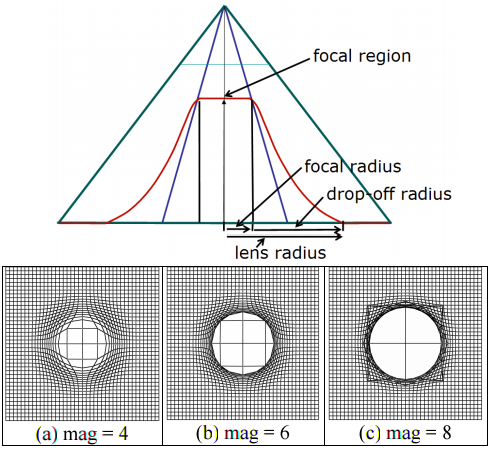
\includegraphics[scale=0.7]{image/LoupeLecture.png}
	\caption{Un aperçu d'une loupe dite de lecture}
	\label{fig:loupeLecture}
\end{figure}

Un des autres types de loupes souvent mis en avant est la loupe dite de lecture. Cette loupe comme visible dans la figure \ref{fig:loupeDemo}, est souvent bornée et cache une partie des informations comme expliqué ci-dessus. On peut voire dans la figure \ref{fig:loupeLecture} un aperçu de ce à quoi peut correspondre une loupe de lecture. On y voit une distorsion d'image sur les bords de la loupe et un ratio fixe de déformation appliqué autour du centre de la loupe (focal region), contrairement aux autres loupes local. Le centre de la loupe fixé et non déformé permet de s'approcher de ce qui est fait aujourd'hui avec des loupes de lecture qui cachent une partie de l'image.

\section{Discussion}

% petit parapgraphe qui reprend les problematiques
% systeme de tracking + deformation
% systeme fisheye a mettre en place
% adapoter l'interaction a la deformation










%
%
%\section{Effet de perspective} 
%
%La perspective est l'un des indices visuels qui nous permet de représenter le monde qui nous entoure. La perspective est un ensemble de règles énoncées par \textit{Filippo Brunelleschi} qui permet de représenter une image sur une surface plane tout en ayant l'impression de réalité grâce à des lignes de fuite. Les lignes sont des ensembles de points qui représentent la direction du plan visualisé. Celles-ci sont présentes lorsque l'on regarde un écran géant de près et donne un rendu étiré de l'image qui est affichée dans notre cas, sur l'écran géant. Voici un aperçu de ce qu'est l'effet de perspective rencontré face à une surface plane, voir \ref{fig:perspectiveScreen}, ce qui est également ce qu'on obtient face aux écrans géants.
%
%\begin{figure}[!ht]
%	\center	
%	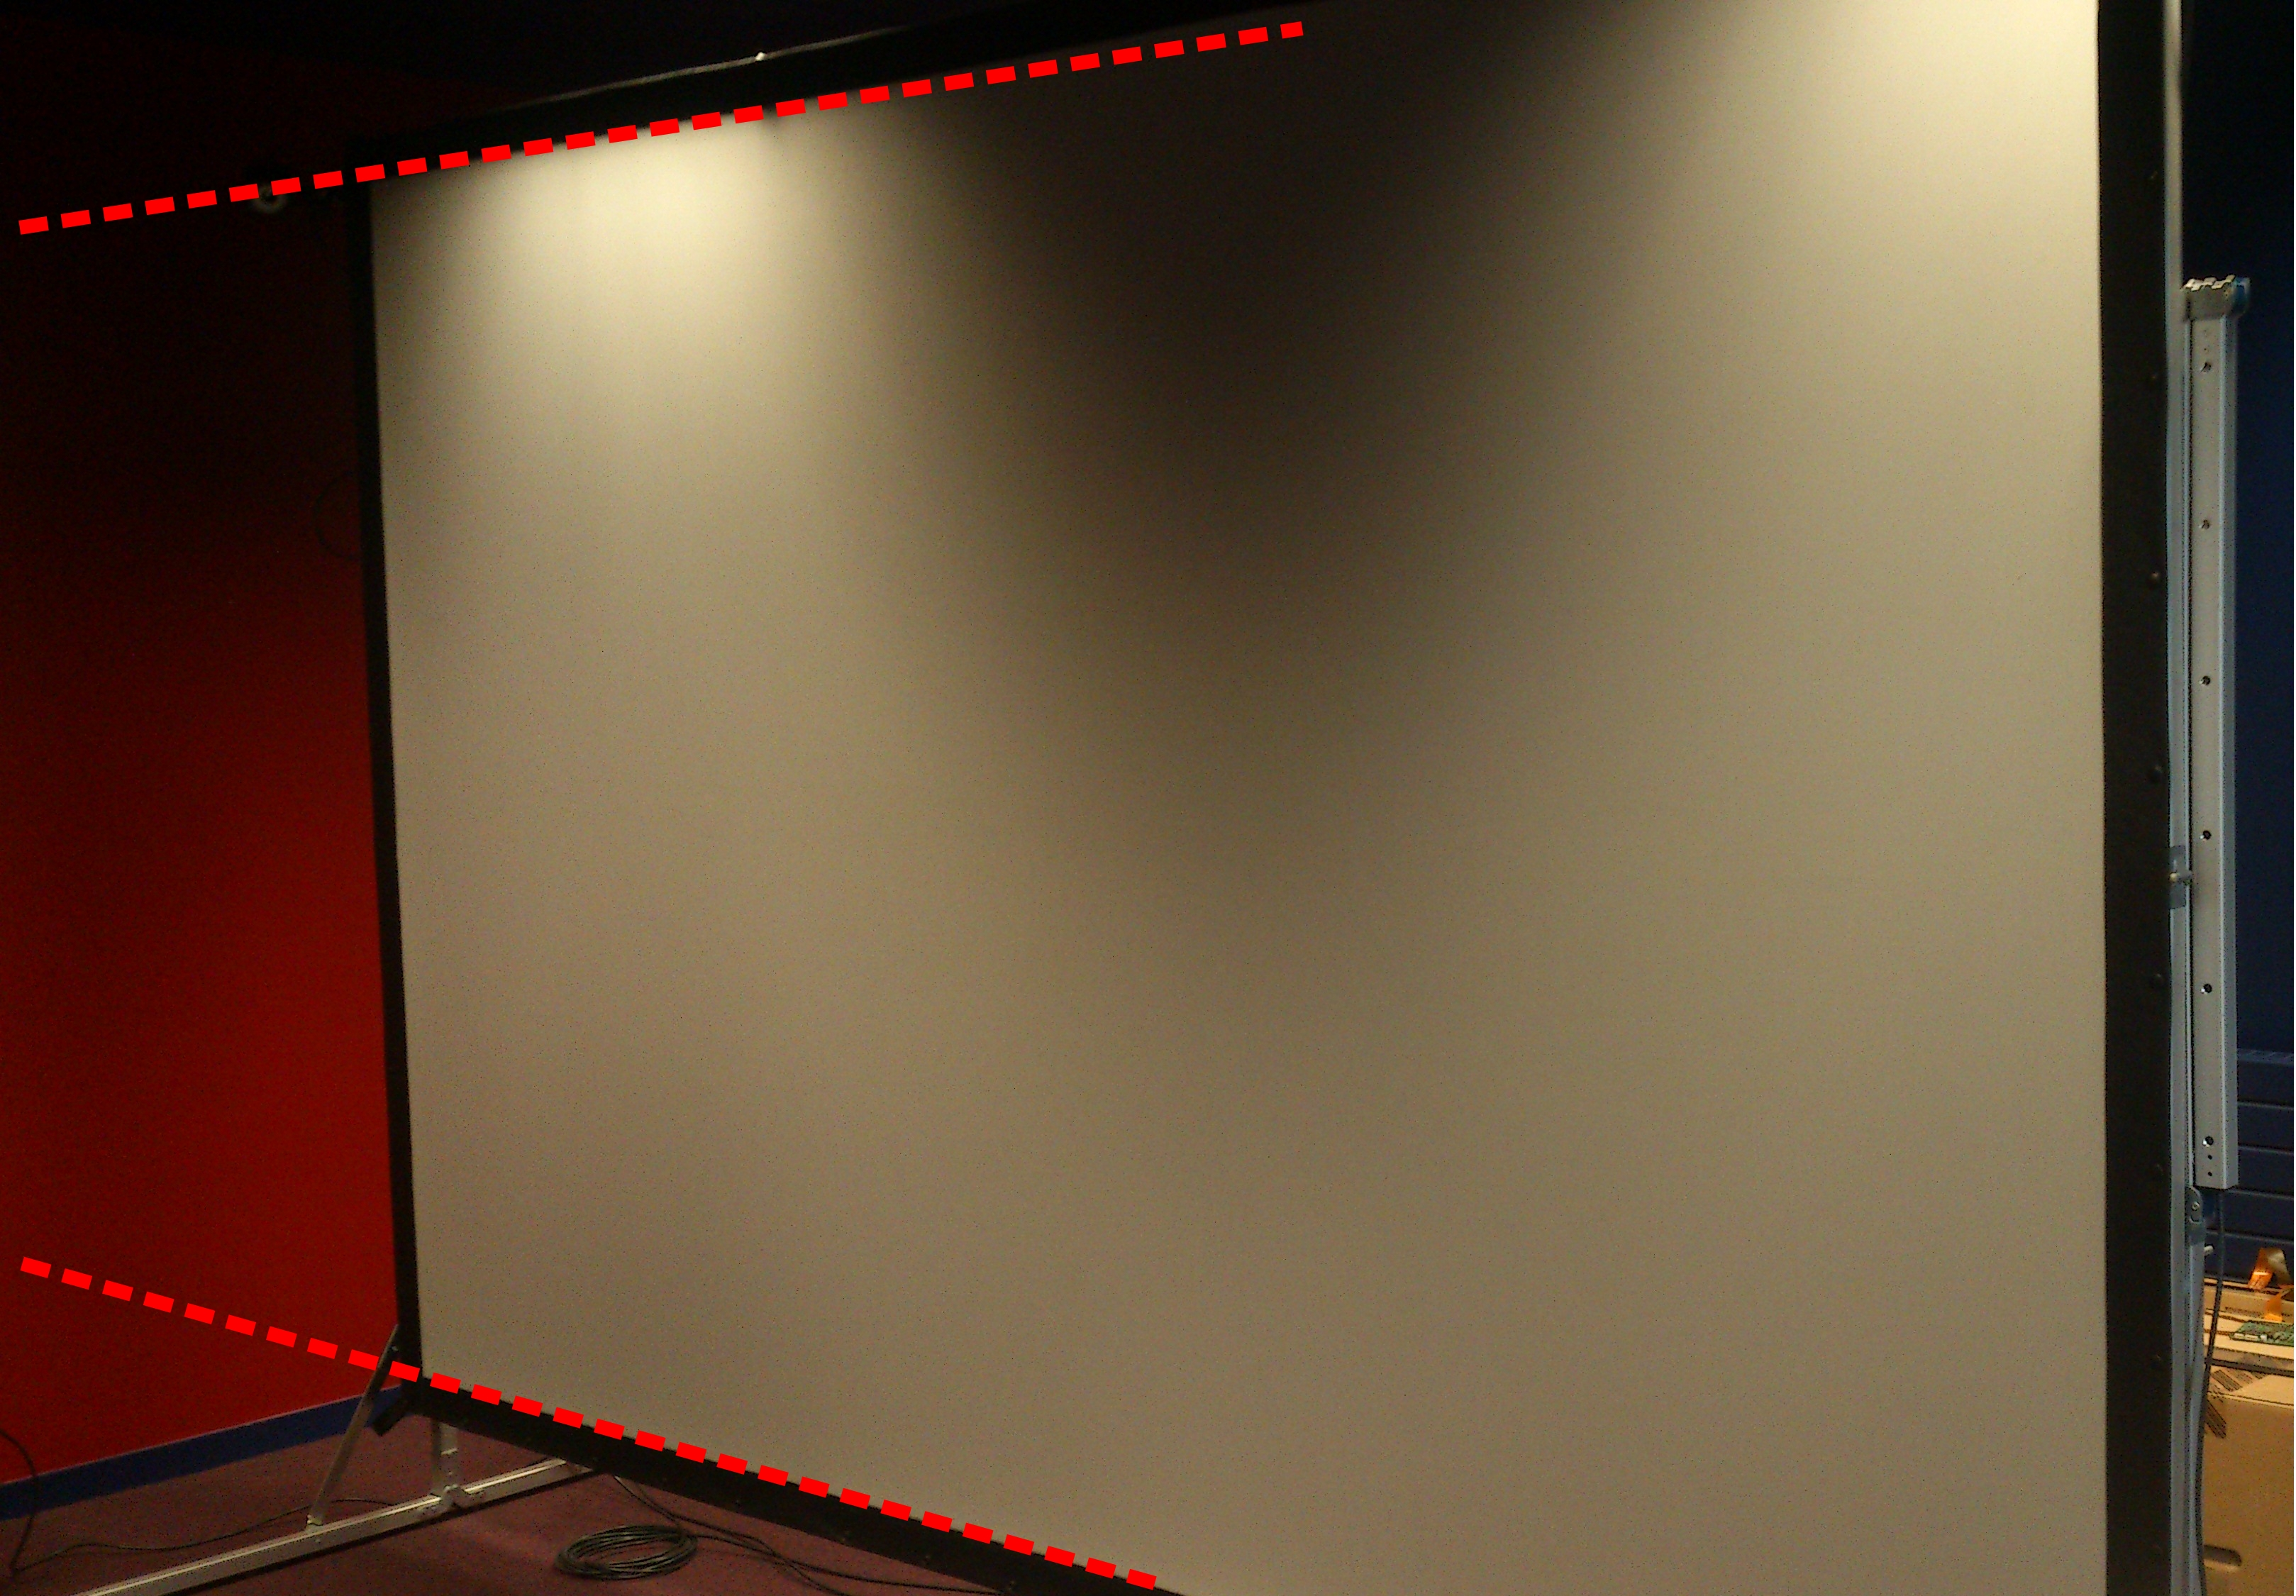
\includegraphics[scale=0.1]{image/perspectiveScreen.jpg}
%	\caption{Effet de perspective visible face à un écran géant}
%	\label{fig:perspectiveScreen}
%\end{figure}
%
%L'effet de perspective est un sujet qui a été traité dans de nombreux cas comme par exemple avec Econics \cite{Nacenta:2007:EPI:1294211.1294260}. Econics est un prototype permettant de définir plusieurs écrans situé a des emplacements et orientation aléatoire tout en proposant pour l'utilisateur un retour visuel de son application orthogonal par rapport à son point de vue et non par rapport à l'écran. Pour réaliser cet effet, ils ont modifié l'apparence visuelle des applications pour corriger l'effet de perspective.
%
%Comme Econics l'a fait pour corriger l'effet de perspective, il est possible de modifier la géométrie des fenêtres affichées de façon indépendante les unes des autres. Une autre solution pour corriger l'effet de perspective serait de déformer l'image complète de l'écran et non uniquement une fenêtre, pour que du point de vue utilisateur tout semble correct. L'anamorphose dynamique est donc envisageable.
%
%\section{Anamorphose, statique et dynamique}
%
%L'anamorphose, dite statique, a été découverte fin du quinzième siècle dans le milieu de l'art tant pour ajouter du challenge aux artistes que pour confirmer leurs maîtrises de la perspective qui fût découverte en même temps.
%Une anamorphose est une déformation réversible d'une image à l'aide d'un système optique, tel un miroir courbe, ou un procédé mathématique.
%
%L'une des plus célèbres anamorphoses est celle réalisée par Hans Holbein sur la toile \textit{Les ambassadeurs}, voir \ref{fig:ambassador}.
%
%\begin{figure}[!ht]
%	\center	
%	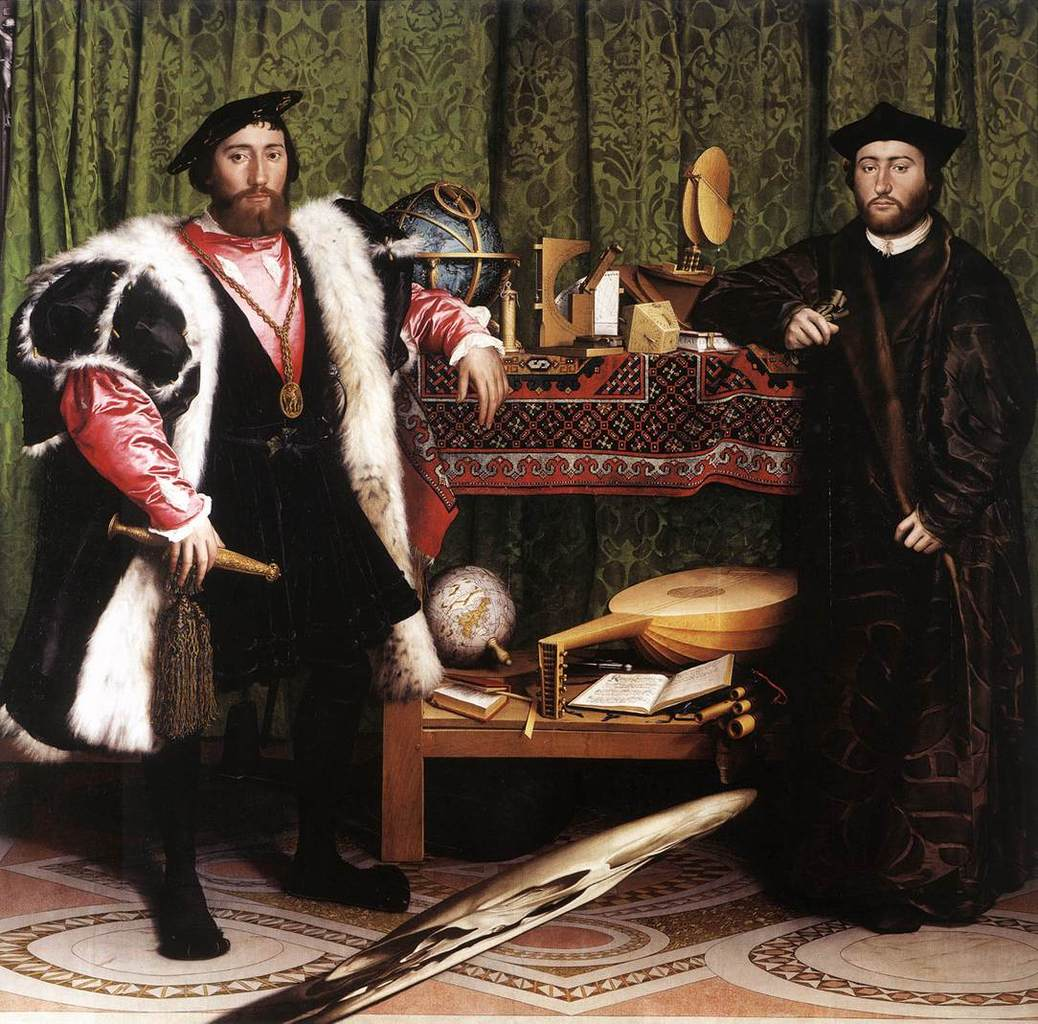
\includegraphics[scale=0.7]{image/ambassador.jpg}
%	\caption{Les ambassadeurs de Hans Holbein le Jeune, 1533}
%	\label{fig:ambassador}
%\end{figure}
%
%Sur cette toile, on peut voir apparaître une forme étrange sur le bas de ce tableau, il s'agit d'une anamorphose d'un crâne humain. Si on regarde le tableau depuis le côté inférieur gauche du tableau, le crane est visible correctement. L'anamorphose est présente sur plusieurs supports, comme par exemple dessiné par des artistes dans certaines rues \cite{pavementArt}.
%
%Dans ce projet nous allons étudier l’anamorphose dite dynamique qui fut introduite par Solina et al. \cite{solina2007dynamic}. L’aspect dynamique de l’anamorphose consiste à ne pas appliquer une déformation statique de l’image, pour laquelle il faut se placer à un point de vue particulier pour obtenir visuellement l'image non déformée, mais déformer l’image en temps réel en tenant compte de paramètres, tels que la position de l’utilisateur face a l’image, pour que celle-ci soit déformée mais parfaitement visible pour l'utilisateur. 
%
%L'anamorphose dynamique introduite par Solina et al. est de la distorsion d'image pour afficher des visages tout en ayant l'impression que le regard des portraits est dirigé vers l'utilisateur. Nous reprendrons donc l'idée de la déformation dynamique sans conserver l'objectif de Solina et al. qui était de garder la direction du regard du portrait vers l'utilisateur.
%
%La correction de perspective a également été mise en place pour le prototype Screenfinity \cite{Schmidt:2013:SEP:2470654.2466227} réalisé par Schmidt et al. . L'objectif de Screenfinity est d'afficher du texte déformé sur un écran géant pour que les passants puissent lire le texte tout en marchant et sans l'effet de perspective. Screenfinity utilise donc la déformation dynamique d'image en tenant compte de la position des passants et de leurs orientation de tête. Pour calculer la déformation à appliquer en fonction de la position et l'orientation des passant, il faut tenir compte de l'acuité visuelle.
%
%\section{Acuité visuelle et modèle de perception}
%
%L'acuité visuelle est la mesure de la résolution spatiale du processus visuel, autrement dit de l'oeil humain. La vision binoculaire est un mode de vision dans lequel les deux yeux sont utilisés simultanément \ref{fig:acuite}. 
%
%\begin{figure}[!ht]
%	\center	
%	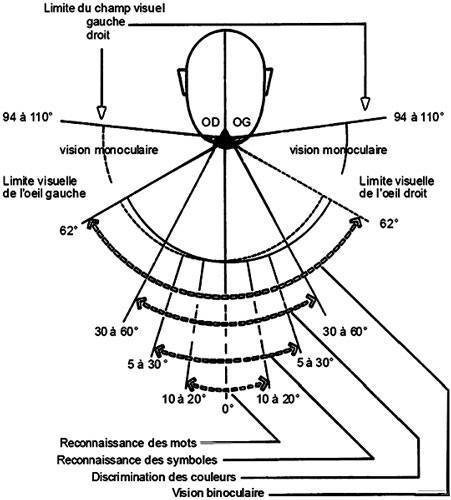
\includegraphics[scale=0.4]{image/acuite.jpg}
%	\caption{Représentation des différents champs de vision de l'être humain.}
%	\label{fig:acuite}
%\end{figure}
%
%Les humains ont un maximum de champ de vision horizontal de $\simeq$180\degres  environ avec les deux yeux, chaque oeil ayant un champ d'environ 150\degres  (90\degres  du côté temporal et 60\degres  du côté nasal) de ce qui permet d'avoir un champ de vision binoculaire de 120\degres  flanqué de deux champs monoculaires d'environ 40\degres. Il donne une sommation binoculaire augmentant la capacité de détecter des objets faiblement lumineux. Il permet une vision stéréoscopique permettant une appréciation précise des distances. En effet, la vision binoculaire est normalement accompagnée de la fusion par le cerveau des deux images perçues par les yeux en une seule mais qui permet d'avoir conscience des distances. 
%
%La vision binoculaire est donc la vue globale qu'un être humain peut avoir. Ce champs de vision sera utilisé pour calculer comment effectuer la déformation de l'image.  
%
%L'acuité visuelle ainsi est également importante dans le cas ou la densité d'affichage est élevé et que l'on souhaite lire à distance des informations. L'une des idées mise en avant est une loupe, ce qui permettra à l'utilisateur de lire à distance l'information voulue sans avoir à utiliser l'outil de déformation d'image qu'il utilisera lorsque celui s'approche de l'écran.
%
%\section{Confort visuel à distance, magnifying glass}
%
%Comme dit précédemment les écrans sont de plus en plus grands et leurs résolutions sont également de plus en plus élevées. Trois problèmes liés à l'augmentation du nombre de pixel présent par unité d'espace, autrement appelé pixel per inch (ppi) sont présentés selon Agarwal et al. \cite{Agarwal:2013:WSA:2578048.2578052}. Sur les trois problèmes identifiés deux nous concernent directement pour l'utilisation distante des grands écrans.
%
%Le premier problème étant que la plupart des applications, les systèmes d'exploitation et plus généralement les interfaces graphiques ne sont pas adaptés pour des résolutions élevées. Ce fut le cas des écrans "Retina" (220 ppi) d'Apple qui ont dû forcer certaines applications à se mettre à jour car inadapté pour une telle résolution, habituellement comprise entre 72 et 110 dpi. Ensuite vient le problème lié à la vision des utilisateurs. En effet les utilisateurs ayant des troubles de la vision, tels que les daltoniens ou encore les personnes âgées, souffrent des mêmes problèmes face à des écrans avec de grandes résolutions d'affichages. Ces problèmes sont des incapacités à lire correctement du texte ou encore à voir avec précision l'ensemble des images affichées à l'écran.
%
%Pour palier à ces problèmes d'affichage trop petit une solution fut d'utiliser les loupes \cite{Kline:1995:IGA:223904.223919}, autrement appelées magnifying glass.
%
%\begin{figure}
%    \centering
%    \subfigure[]{\label{sub1} 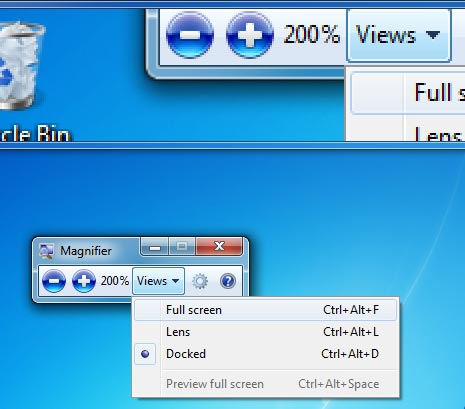
\includegraphics[scale=0.4]{image/loupeWindows.jpg}}
%    \subfigure[]{\label{sub2} 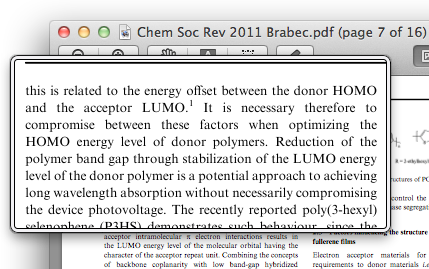
\includegraphics[scale=0.4]{image/loupeMac.png}}
%    \caption{Aperçu des loupes implémentés dans \subref{sub1}Windows et \subref{sub2}Mac OS X.}
%	\label{fig:loupeDemo}
%\end{figure}
%
%Parmi les loupes existantes et implémentées dans les systèmes d'exploitation modernes, la plupart occupent l'ensemble de l'écran ou cachent certaines parties autour de la loupe, voir figure \ref{fig:loupeDemo}. Cela à pour effet de perdre une partie des informations se trouvant sous les bords de la loupe. Pour les loupes qui occupent une plus grande partie de l'écran, cela a pour effet de perdre encore plus d'informations car si l'utilisateur n'a pas connaissance de son environnement graphique, il doit parcourir l'ensemble de l'écran pour pouvoir s'y repérer et interagir. 
%
%Pour garder une vue globale de l'environnement graphique de nombreuses loupes ont étés expérimentés \cite{Carpendale:2004:AHM:1029632.1029645}. L'une des loupes qui ré-apparaît souvent dans la littérature est la loupe fisheye
%
%Dans le domaine de l'interaction homme machine la question du zoom fisheye a souvent été étudié \cite{Shneiderman:1986:DUI:6682, Ware:1995:DIM:223355.223749, Cockburn:2009:ROZ:1456650.1456652} et mis en avant pour montrer l'avantage de cette technique en ce qui concerne la mise en focus de certains éléments. L'une de ses utilisations la plus connue est sur le dock de max OS X. L'effet fisheye est une distorsion de l'image qui apporte un gain de performance \cite{Bederson:2000:FM:354401.354782, Furnas:1999:FVN:300679.300769, Gutwin:2002:IFT:503376.503424, Gutwin:2003:FGL:642611.642648} lorsque l'utilisateur souhaite parcourir des données et se concentrer sur une de ces données. Cependant lors d'une sélection, l'effet de distorsion affecte positivement le nombre d'erreurs \cite{Gutwin:2002:IFT:503376.503424}. L'effet fisheye apporte donc une loupe dite contextuelle.
%
%Un des autres types de loupes souvent mis en avant est la loupe dite de lecture. Cette loupe comme visible dans la figure \ref{fig:loupeDemo}, est souvent bornée et cache une partie des informations comme expliqué ci-dessus. XXXXXXXXXX \cite{} qui a expérimenté un ensemble de loupe montre qu'une loupe de lecture avec une distorsion d'image sur les bords de la loupe et un ratio fixe de déformation appliqué autour du centre de la loupe peut correspondre à ce qui est actuellement fait pour les loupes de lecture.

\chapter{Hypothèses de travail}

\section{ARTrack}

L’ARTrack  pour Advanced Realtime Tracking est un ensemble de caméra infrarouge développé par la société Vicon. Ces caméras fonctionnent grâce à des marqueurs. Il est possible de traquer avec précision n’importe quel élément équipé de trackers. 

\begin{figure}[!ht]
	\center	
	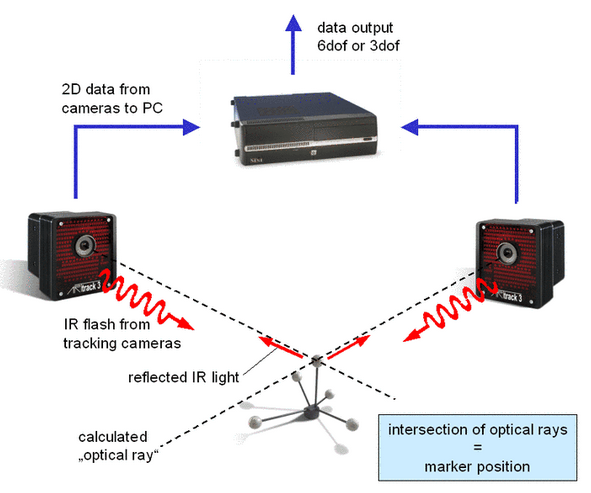
\includegraphics[scale=0.5]{image/artrack.png}
	\caption{ARTrack}
\end{figure}

Cette solution présente plusieurs avantages. Premièrement la précision, les ARTracks sont des caméras permettant de tracker n’importe quoi avec une grande précision. Tracker la position de la main de l’utilisateur ainsi que le support physique seront suivis avec énormément de précision. Une pièce configurée avec un ensemble de caméra ARTrack pourrait permettre de résoudre les problèmes de précision mais également d’obstruction.

Cependant nous souhaitons mettre en oeuvre une solution disponible au grand public. Les ARTracks étant un équipement coûteux et complexe dans son installation ainsi que dans sa  calibration, cette technologie ne peut pas utilisé dans le cadre d’une application grand public.

\section{Tag}

Pour tracker facilement un objet, nous pouvons lui ajouter des QR Codes. Les QR Codes sont un type de codes barres à deux dimensions. Il est aujourd’hui l’un des codes bidimensionnels les plus utilisés. Il sont en effet utilisés pour rediriger vers un site internet ou encore pour afficher du contenu multimédia.

\begin{figure}[!ht]
	\center	
	
\includegraphics[scale=0.25]{image/qrcode.png}
	\caption{QrCode}
\end{figure}

L’utilisation des QR Codes permettrait donc de différencier les objets physiques lambda et le support physique sélectionné pour interagir. De plus en utilisant les QR Code il serait possible d’utiliser différents types d’interaction en fonction du support sur lequel on plaque le QR Code. Par exemple, on pourrait définir un QR Code pour un bloc note et, dès le début de l’interaction, un éditeur de texte pourrait s’ouvrir pour prendre en note l’écriture de l’utilisateur. Cela permettrait également d’obtenir la position exacte et l’orientation de l’objet. 

Cependant cette solution ne sera pas retenue car nous souhaitons une application grand public sans aucune contrainte, cf pose des QR Code sur les supports.

\section{Solution multi-Kinect}

Étant donné que notre problème principale est que, lorsque le support physique est à la verticale, le champ de vision de la Kinect est obstrué par celui-ci. On peut donc penser à utiliser plusieurs Kinects pour éviter les angles mort. 

La logique est simple, l’utilisateur se met face à la Kinect principale pour que celle-ci l’identifie et analyse ses mouvements. Une fois que la Kinect principale a trouvé l’emplacement de l’utilisateur, la deuxième Kinect analyse les mouvements de celui-ci et les données des deux Kinects sont fusionnés pour plus de précision. 

Grâce à cette deuxième Kinect, lorsqu’un objet est présent entre l’utilisateur et la Kinect ou lorsque le support physique est vertical, la deuxième Kinect permet de récupérer quand même le mouvement et donc l’application fonctionne toujours.
	
Le problème est que l’utilisation de deux Kinect en stéréovision est compliqué et que cela nécessite une bonne configuration des Kinect. Un calibrage important est nécessaire .


\section{Kinect en hauteur}

Une possibilité pour pouvoir éviter l’occlusion causée par le support physique serait de mettre la caméra Kinect en hauteur. Celle-ci bénéficiera d’un point de vue qui permettra une plus grande liberté dans le placement du support physique par l’utilisateur.

\begin{figure}[!ht]
	\center	
	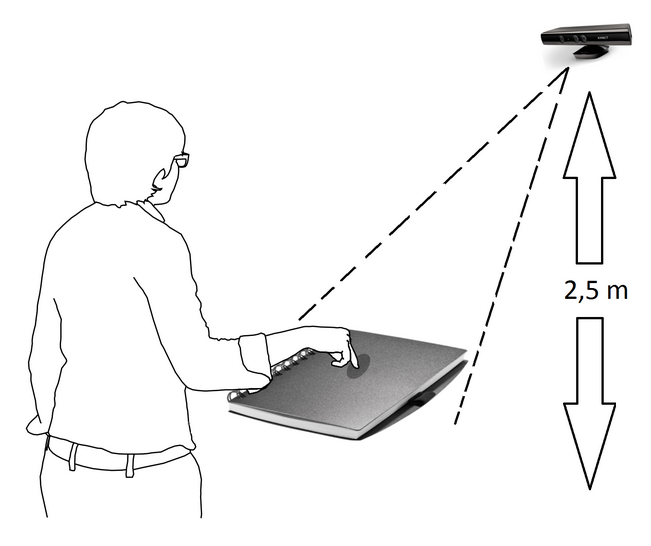
\includegraphics[scale=0.25]{image/result.png}
	\caption{Proposition de placement de la Kinect}
\end{figure}

Certes, cette solution n’est pas idéale dans le sens que, l’occlusion sera toujours possible puisque nous restons dans un environnement visuel à deux dimensions. Elle reste pour autant la solution la plus abordable pour le grand public puisque, une et une seule Kinect est nécessaire ce qui facilite l’intégration. Cependant certaines conditions d’installations seront à respecter, tels que la hauteur de la Kinect ou encore son angle d’orientation.

\chapter{Répartition des taches}

La mise en oeuvre de notre projet se déroulera selon 4 composantes principales. 
Dans un premier temps nous commencerons par nous familiariser avec le code existant. Cette étape consiste à comprendre le mécanisme de l'application et de refactorer le code source. En parallèle une partie de notre équipe s'occupera de faire des tests et de régler la Kinect.

Une fois cette première partie finie, nous commencerons l'implémentation de notre solution. Notre premier objectif sera la reconnaissance du support suivit du tracking de la main sur celui-ci. Enfin nous étendrons l'application à une solution  multi-utilisateur.

Au cours de cette seconde partie nous commencerons la rédaction du rapport technique. Le projet étant terminé à ce stade, nous nous concentrerons sur la soutenance ainsi que sur d'éventuelles améliorations dîtes facultatives. Nous pensons notamment à tester l'implémentation d'une solution multi-kinect ou encore la solution ARTrack.

Un diagramme de Gantt récapitulatif se truove en annexe.
\chapter{Conclusion}

Nous avons vu dans ce rapport la phase d'analyse de notre projet. Celui-ci consiste en l'amélioration d'une application de tracking existant permettant le contrôle de la souris. 

Nous avons examiné plusieurs solutions pour corriger le problème de non visualisation de l'espace d'interaction et du manque de retour physique tout en rendant l'application multi-utilisateurs. Pour répondre à ces problèmatiques, nous avons étudié plusieurs solutions telles que l'utilisation d'ARTrack ou d'utiliser plusieurs Kinect. 

Comme nous souhaitions rendre l'application grand public, nous avons préféré opter pour une solution n'utilisant qu'une seule Kinect, celle-ci sera positionnée en hauteur avec un angle spécifique pour permettre d'observer le support sans avoir d'oclusions selon l'angle du support. 

Maintenant que la partie analyse est accomplie, nous allons pouvoir commencer l'implémentation de notre solution. Cependant, il est possible que certaines difficultés apparaissent en cours de projet. Notamment, l'absence de retour d'information concernant la réussite du tracking de l'objet support.
\chapter{Glossaire}

\textbf{Kinect} Il s'agit d'une caméra utilisant des techniques d'interaction développées par la société israélienne PrimeSense, longtemps nommée par le nom de code du projet, "Project Natal", elle a été officialisée juste avant l'E3 sous le nom Kinect. Elle est basée sur un périphérique d'entrée branché sur la console Xbox 360 qui permet d'interagir par commande vocale (pas disponible au lancement en France), reconnaissance de mouvement et d'image.\\

\textbf{Tracking} est l'ensemble des moyens mis en oeuvre pour suivre, dans
notre contexte, un corps en mouvement.\\

\textbf{ARTrack} L’ARTrack (Advanced Realtime Tracking) est un ensemble de caméra infrarouge développé par la société Vicon. Ces caméras fonctionnent gráce a des marqueurs. Il est possible de traquer avec précision n’importe quel élément équipé des trackers.\\

\textbf{QR Code} Les QR Codes sont un type de codes barres à deux dimensions.\\

\textbf{SDK} Un SDK (Software Development Kit) est un ensemble d'outils permettant aux développeurs de créer des applications.

\bibliography{Bibliography}

\pagestyle{empty}
\begin{figure}[!ht]
\chapter{Annexes}
	\center	
	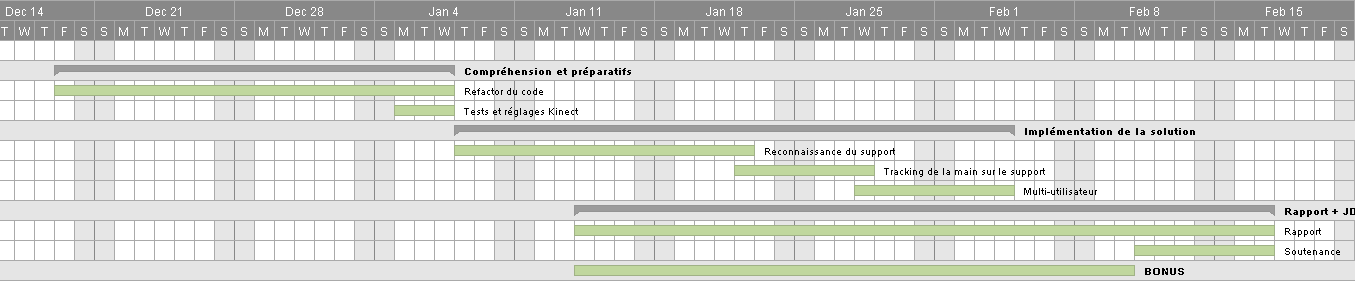
\includegraphics[scale=0.4,angle=90]{image/gantt.png}
	\caption{Diagramme de Gant des tâches}
\end{figure}
%%%%%%%%%%%%%%%%%%%%%%%%%%%%%%%%%%%%%%% contenu futur

\newpage
%\chapter*{Résumé}

TODO ?


\end{document}